\documentclass{article}
%     % General document formatting
    \usepackage[margin=0.7in]{geometry}
    \usepackage[utf8]{inputenc}
    \usepackage{tabularray}
    \usepackage[fontsize=12pt]{fontsize}
    \usepackage[parfill]{parskip}
    \usepackage{hyperref}
    \usepackage[final]{listings}
    \usepackage[T1]{fontenc}
    \usepackage{listings}
    \usepackage{xcolor}
    \usepackage{graphicx}
    \usepackage{float}
    \usepackage{titlesec}

\title{%
    Opening various image formats\\
    \large Software Maintance Autumn 2023
}
\author{Magnus Christian Larsen}
\lstset{breaklines=true, captionpos=b, numbers=left, numberstyle=\color{gray}, tabsize=2, backgroundcolor=\color{gray!10}}



\begin{document}
\maketitle
\vspace*{\fill}
\begin{center}
    \bf{%
        GitHub Username: Autowinto\\
        Student Mail: magla21@student.sdu.dk\\
        Project: https://github.com/Autowinto/JHotDraw\\
        Date: mm/dd/yyyy}
\end{center}
\newpage
\tableofcontents
\newpage

\section{Change Request}
From the list of features that were available to be implemented, in the group, it was decided, that I would be implementing the "open various formats" feature. This includes png, jpg, gif, pct and text. 

\subsection{User Story}
The change request, defined as a user story, is as follows:

\textbf{"As a user, I want to be able to open images of the formats png, jpg, gif, pct, and text, so that I can work with many different formats without having to convert myself"}

\subsection{Acceptance Criteria}
The following subtasks as identified serve as acceptance criteria:
\textbf{%
\begin{itemize}
    \item When I click on the 'Open' option, the software should allow me to browse and select files in png, jpg, gif, pct, and text formats.
    \item Upon selecting a valid file of the mentioned formats, the software should display the image or content correctly within the workspace.
    \item If I attempt to open a corrupted or unsupported file type, the software should provide a clear error message.
    \item The software should maintain the original quality of the image when opening it.
    \item For text files, the software should provide an option to convert the text into an editable shape or object in the drawing workspace.
\end{itemize}
}
\section{Concept Location}
\subsection{General Methodology}
In locating classed for the refactoring process of the report, there are several options available to us within Featureous and NetBeans, which we of course will make use of in the future impact analysis section of the report. For actually finding the location of classes relevant to the feature, I mainly made use of the powerful tools provided by the IntelliJ IDE, such as the following:

\begin{itemize}
    \item Find usages - Allows you to find usages of any given method or variable
    \item Go to implementation - Allows you to go directly to the implementation of a method
    \item Search within file - Allows you to search for any symbol or token within a single file.
    \item Inspect code - Allows you to see a bunch of metrics about code such as maturity, implementation issues and more, helping to pinpoint problematic parts of the code.
\end{itemize}

In addition to tooling provided by NetBeans and IntelliJ, there are also methods that are much less technical, such as simply removing parts of the code and seeing what happens and if said code is relevant to the feature that is being refactored.

\subsection{Classes Overview}

\begin{center}
    \begin{tblr}{hlines, vlines}
        \bf{\#} & \bf{Domain classes}       & \bf{Tool used} & \bf{Comments} \\
        1       & LoadFileAction            &                &               \\
        2       & OpenFileAction            &                &               \\
        3       & AbstractApplicationAction &                &               \\
        4       & AbstractAction            &                &               \\
    \end{tblr}
\end{center}

Use Featureous Feature call-tree to provide a tree-based visualization of the runtime call graphs of methods implementing the features of your change request. This view provides an execution- based alternative to the hierarchical fashion of browsing features supported by the mentioned feature inspector view.

\section{Impact Analysis}
An impact analysis serves the purpose of helping a developer understand the implications and impact of performing a refactor or introducing a feature into a software project. This is especially relevant, as the group consists of 5 total members, each refactoring their own feature, which could very quickly result in overlapping code changes, code constantly breaking and the end product becoming unstable.

To perform this impact analysis, we're making use of the program featureous and FeatureEntryPoint annotations to annotate parts of the program that is planned to be refactored. By doing this, we can gain a further understanding of the interconnectivity of the program and see how the features overlap code-wise.

The FeatureEntryPoints created for my feature are for the following methods and constructors.

\begin{itemize}
    \item OpenFileAction constructor
    \item OpenRecentFileAction constructor
    \item actionPerformed in OpenFileAction.java
    \item openViewFromURI in OpenFileAction.java
    \item showDialog in OpenFileAction.java
    \item createDialog in OpenFileAction.java
\end{itemize}

Based on these FeatureEntryPoints, the generated report can be used to analyze the impact of the feature.

\subsection{Featureous Feature-Code Characterization}
\begin{figure}[H]
    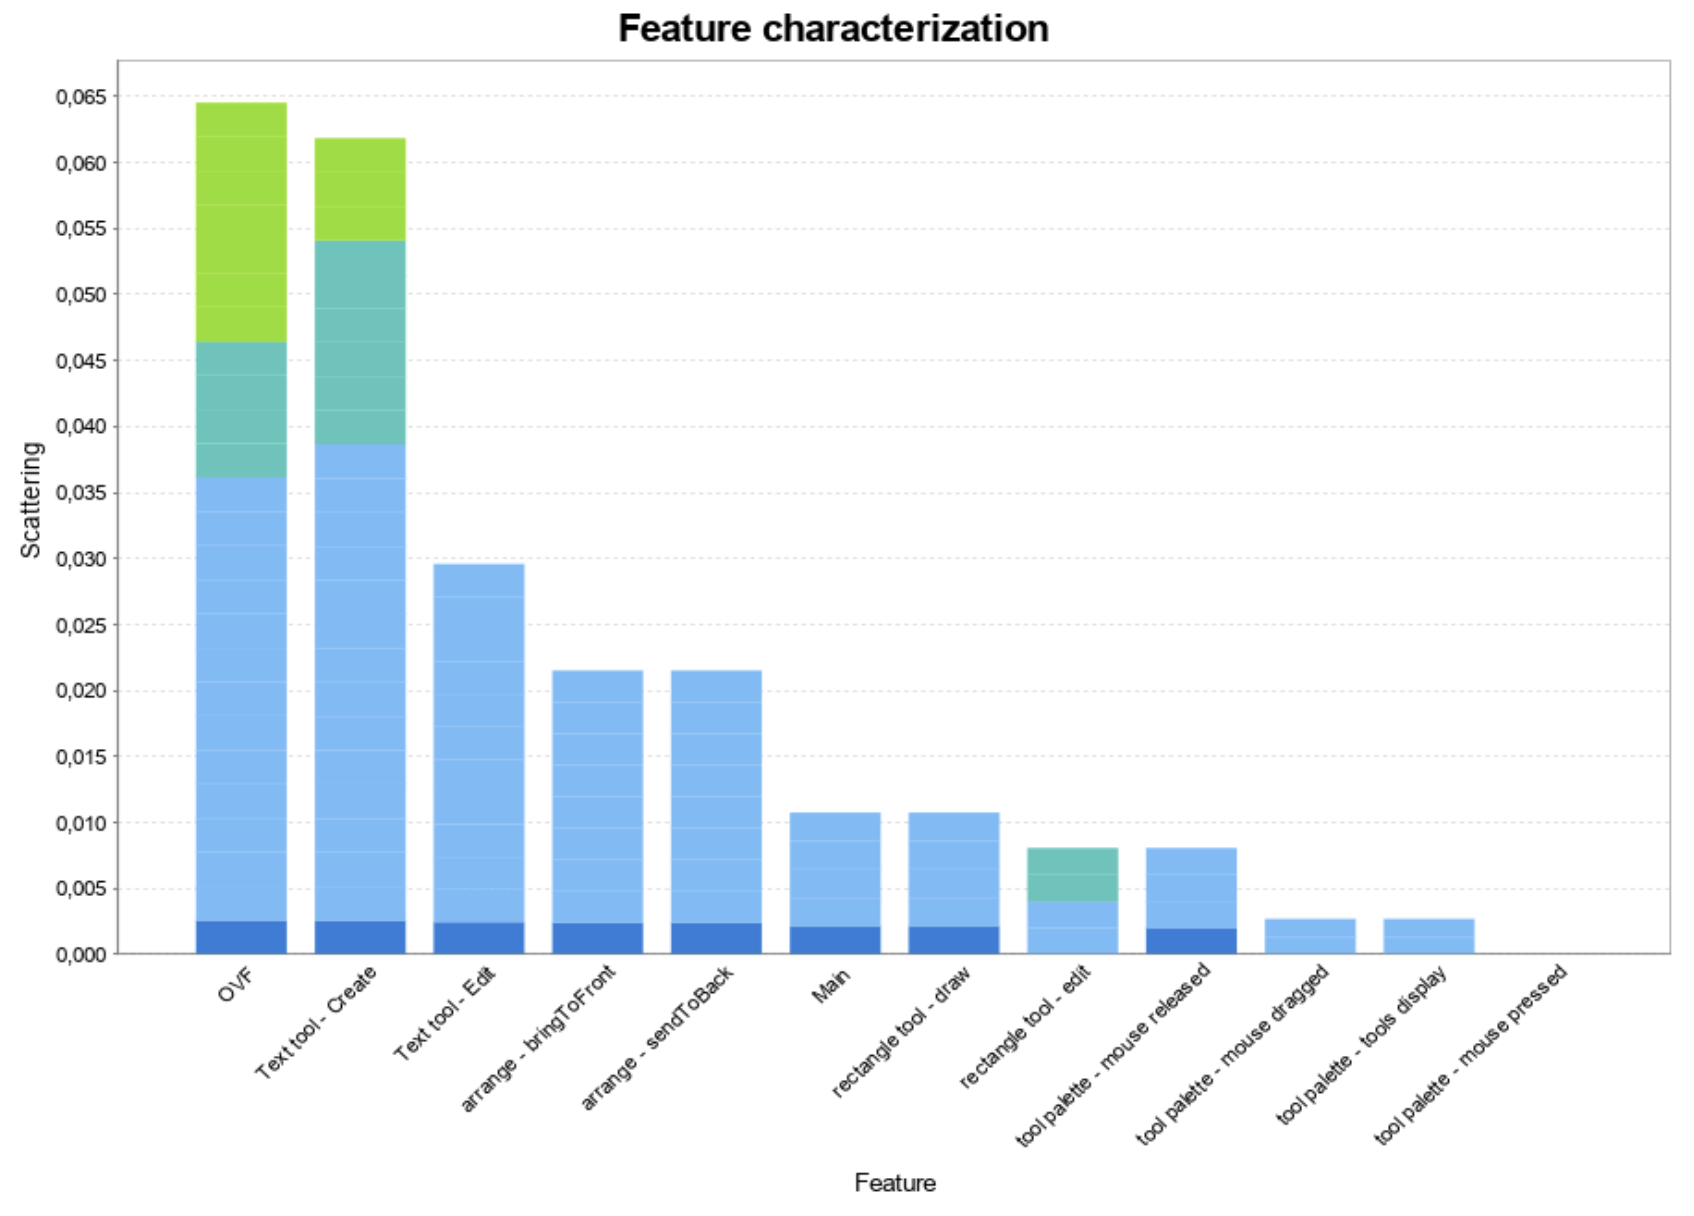
\includegraphics[width=\textwidth]{Images/featurecharacterization.png}
    \caption{Feature-Code Characterization}
\end{figure}
The above graph from featureous shows that my feature, here annotated as OVF, has a great deal of overlap with other features and is very scattered in the codebase. This means, that when refactoring, I need to be extra careful not to accidentally break other features, causing additional refactoring between me and another team member to be necessary.

\subsection{Feature Correlation Grid}
\begin{figure}[H]
    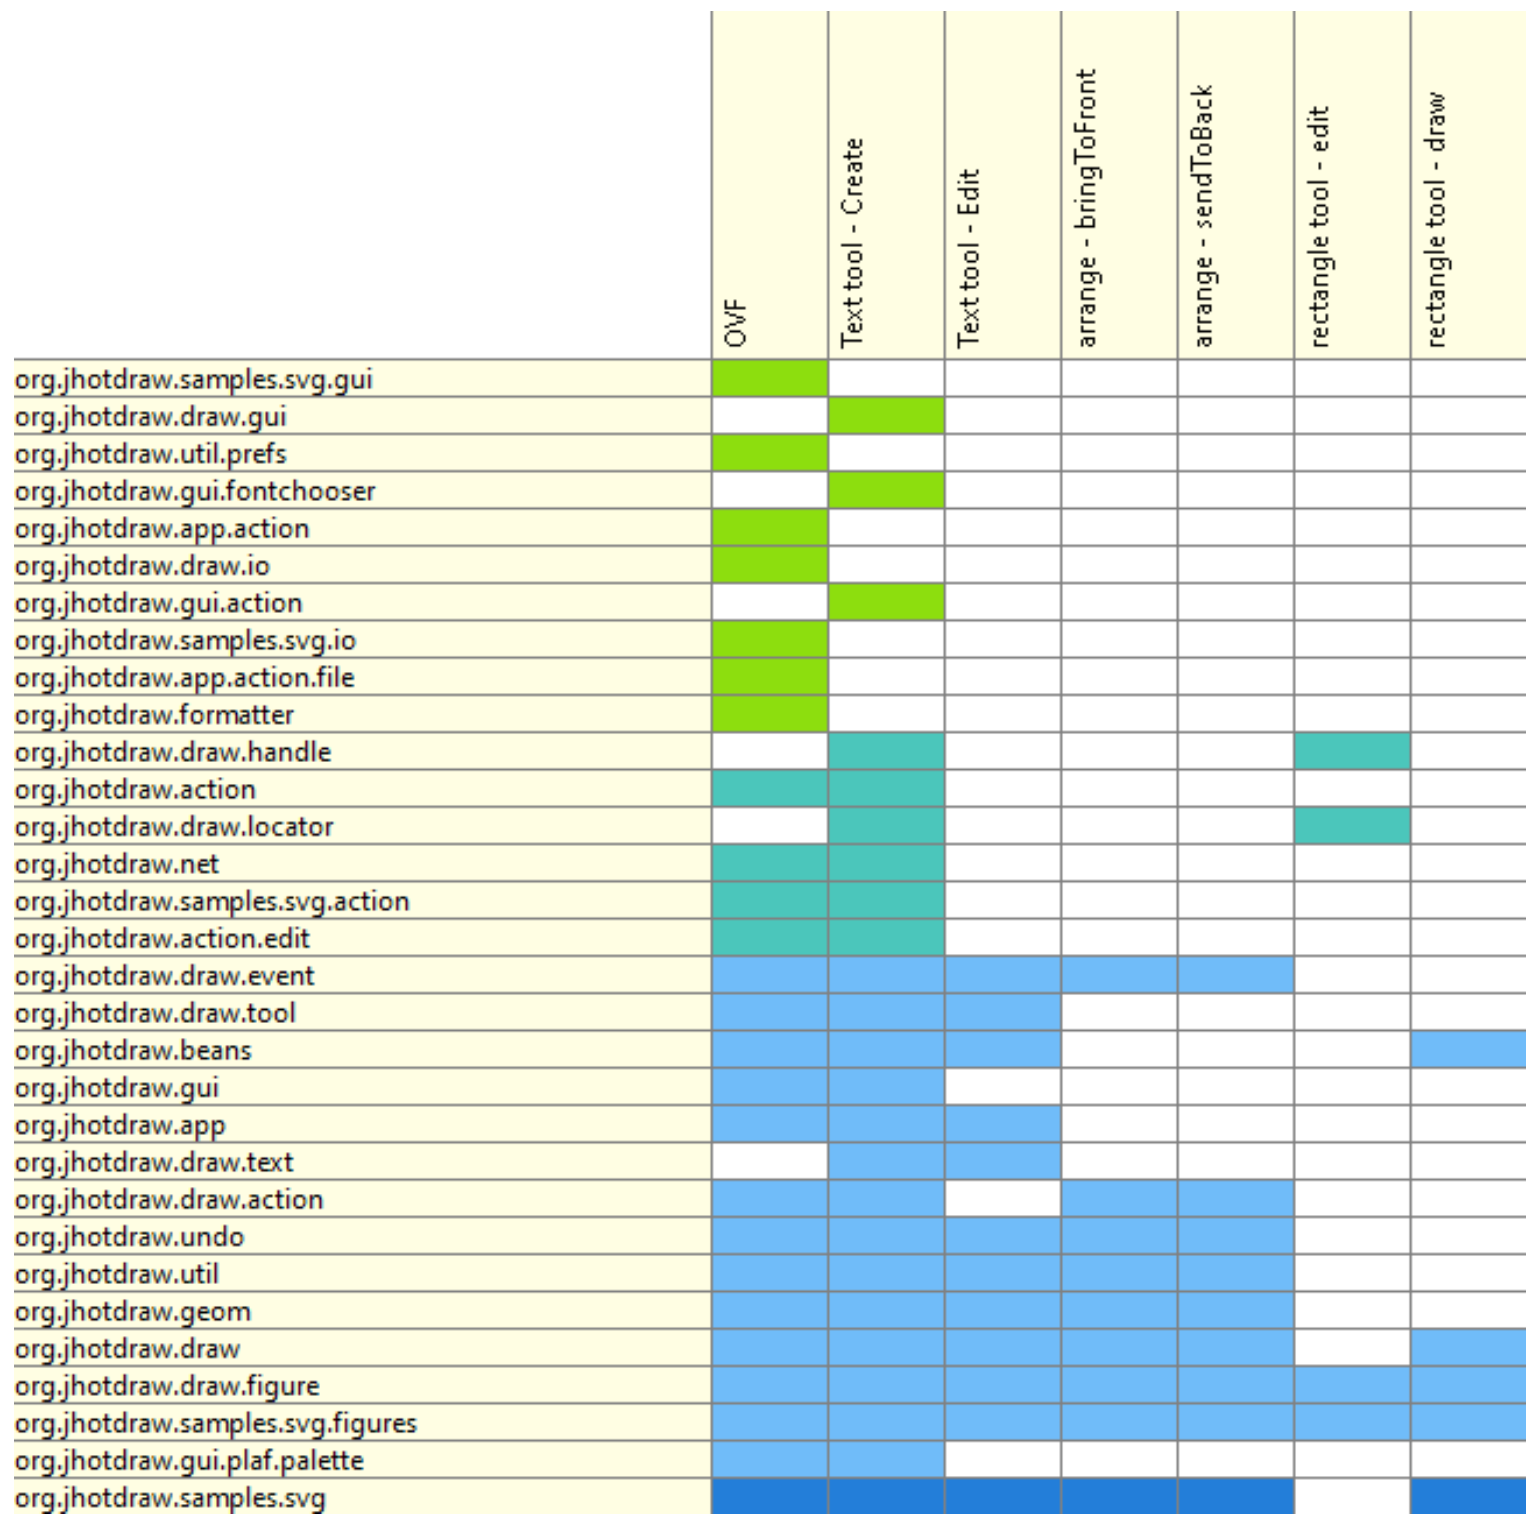
\includegraphics[width=\textwidth]{Images/featureousgrid.png}
    \caption{Feature Correlation Grid}
\end{figure}
Reading the grid reveals, that my feature has great entanglement with other features. There are several reasons why this could be the case. Firstly, my feature handles many things. Performing IO to load files, placing these image files in the GUI, drawing said feature on the screen and more. Therefore, the entanglement on display doesn't necessarily mean, that refactoring will be difficult; it does however show, that we should be wary when refactoring and extra careful that core features aren't broken when refactoring.

\subsection{Feature Correlation Graph}
\begin{figure}[H]
    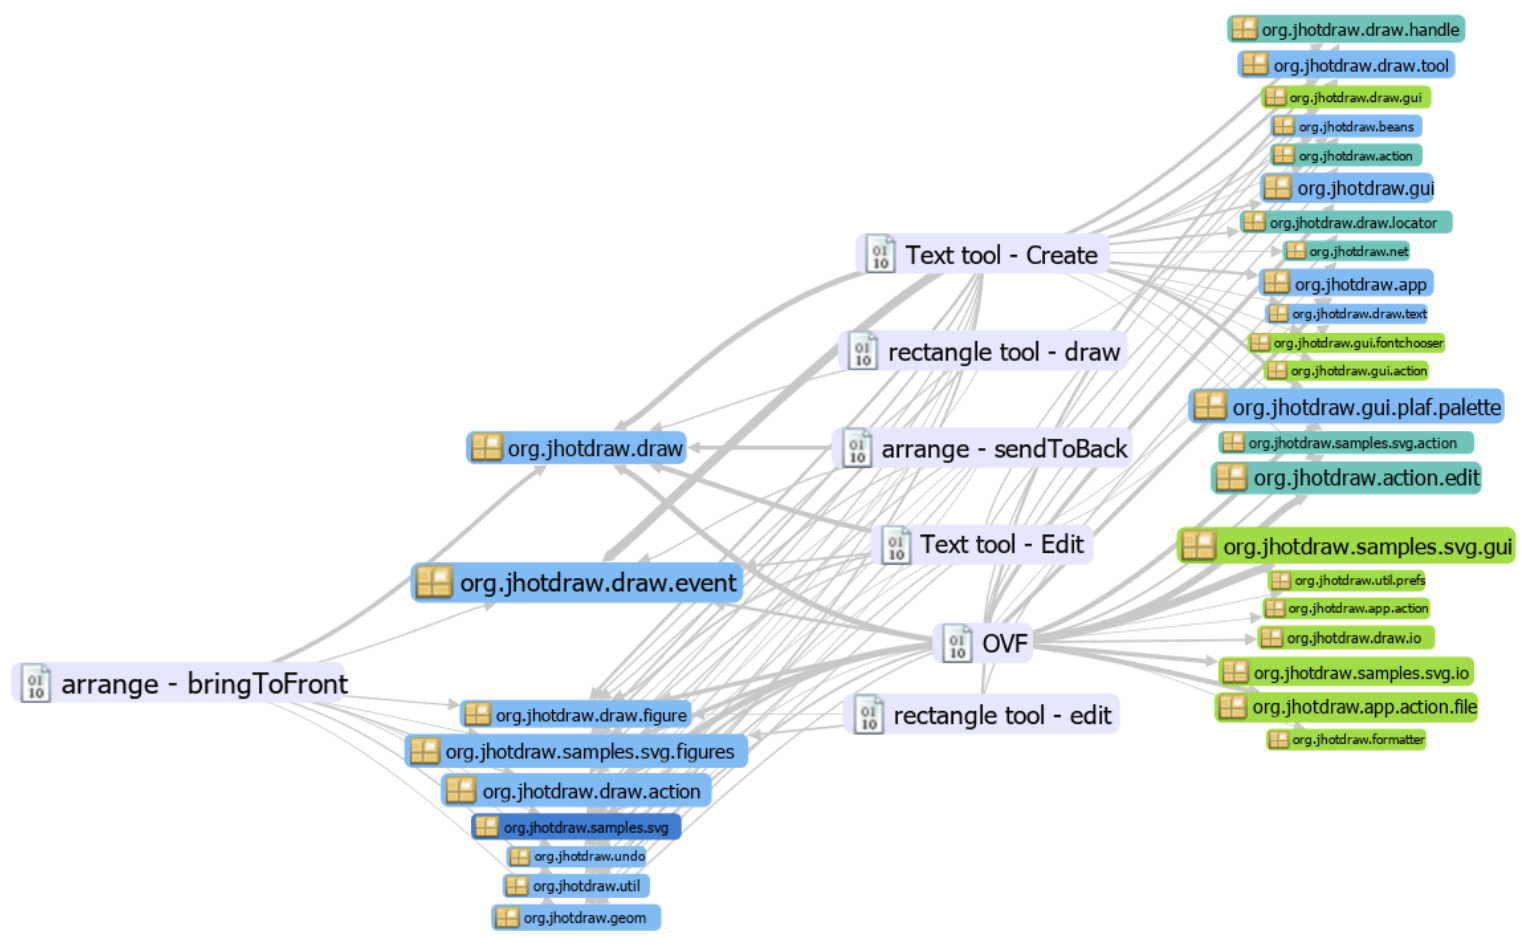
\includegraphics[width=\textwidth]{Images/featureousgraph.png}
    \caption{Feature Correlation Graph}
\end{figure}
The graph generated by the Featureous doesn't give us a lot of new information, it does however present it in another way, which gives further evidence to the fact, that while the code overlap previously seemed to be deeply ingrained, the overlaps happen in key packages such as the draw event package, figures, action etc. many of which, we won't be touching for the coming refactor or will be extra careful not to break.

\subsection{Feature Relations Characterization}
\begin{figure}[H]
    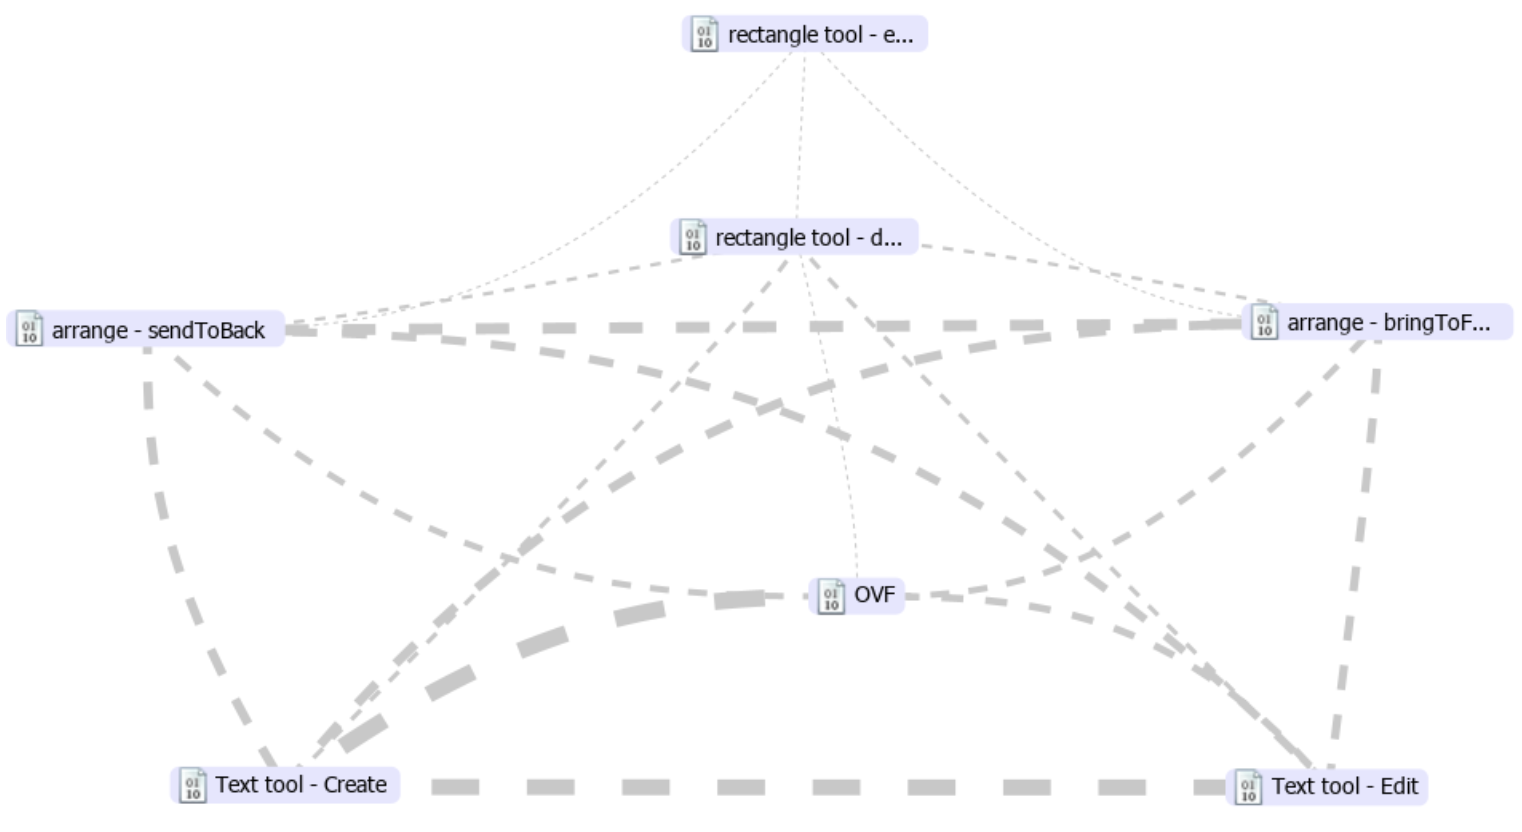
\includegraphics[width=\textwidth]{Images/featureousrelations.png}
    \caption{Feature Relations Characterization}
\end{figure}

Yet another visualization tool of the Featureous software, is the feature relations characterization, which is a simpler visualization, showing the amount of shared relations between the different features with a dashed line, increasing in thickness directly proportional to the amount of shared code. This is helpful if, like our feature correlation graph, the amount of packages on display is hard to read.

While a useful tool in many contexts, in my case, I feel it doesn't help me a lot, as my feature seemingly connects to most other features in one way or another and doesn't help me gain an entry point into analyzing my feature's impact.

\subsection{Impact Analysis}
The impact of the feature that I will be refactoring can be broken down in a table of classes and packages, helping with a general overview of the things that I need to be wary of when refactoring. These will be marked by one of the three following tags.

\begin{itemize}
    \item \textbf{Unchanged}: These are classes that I visited in my search for relevant classes, but will not be touching.
    \item \textbf{Propagating}: These are classes that I looked at, and helped me find the correct classes that I was looking for.
    \item \textbf{Changed}: These are classes that I have planned to refactor based on my analysis.
\end{itemize}

% TODO: FILL THIS OUT
\begin{longtblr}[caption = {The list of all the packages visited during impact analysis.}]{|l|l|l|l|}
    \hline
    \bf{Package name} & \bf{\# of classes} & \bf{Tool used} & \bf{Comments} \\
    \hline
    \bf{action}       & \bf{}              & \bf{}          & \bf{}         \\
    \hline
    \bf{action.file}  & \bf{}              & \bf{}          & \bf{}         \\
    \hline
    \bf{action.app}   & \bf{}              & \bf{}          & \bf{}         \\
    \hline
    \bf{}             & \bf{}              & \bf{}          & \bf{}         \\
    \hline
\end{longtblr}

\section{Refactoring Patterns and Code Smells}

%There is so much fucking duplicated code.
%The methods are incredibly long
%Method names are fucked and have no proper meaning
%Long parameter lists
%Confusing naming of classes and functions.

%There is no reason to be abbreviating variables to the point of them being single letters. It makes for confusing code, especially in longer methods.

%Describe the code smell that triggered your refactoring, see Chapter 4 in [Ker05].
%Describe what you plan to change by refactoring.
%Why do you think it's good to do the refactoring?
%Describe the strategy of the refactorings. Remember there is not one way to implement a pattern.
%Which of the refactorings from [Ker05] did you apply and what was the reasoning behind it?

The class that are gonna be the focus of the upcoming refactor is the OpenFileAction class. In order to find relevant code smells, I made use of the SonarLint plugin for IntelliJ, which is specially created to identify non-critical code smells in code, helping to improve clarity and maintainability of the code written.

\subsection{Duplicated Code}
The two files are similar in functionality. Unfortunately, they are also very similar in code, violating the DRY principles\footcite{kerievsky}, as they each have plenty of code that is duplicated across the clas that could very well be refactored into some shared class or helper methods. An example of this can be seen below with two code snippets from OpenFileAction and OpenRecentFileAction respectively that has almost identical code for finding an empty view.
\begin{figure}[H]
  \lstinputlisting[language=java, firstline=103, lastline=119]{Code/OpenFileAction.java}
  \caption{OpenFileAction.java}
\end{figure}

\begin{figure}[H]
  \lstinputlisting[language=java, firstline=84, lastline=98]{Code/OpenRecentFileAction.java}
  \caption{OpenRecentFileAction.java}
\end{figure}

This also isn't the only example of duplicate code being employed. In fact, the two classes are more or less identical and could greatly benefit from this refactor.

\subsubsection{Refactoring Strategy}
The strategy that we'll be employing to refactor the class, is to move the shared code into some kind of shared location or utility class, so that we reduce the size of the classes themselves and have an easier time splitting up the code. Additionally, as there are many action classes, future refactors could benefit from these utility classes as well.

It's also a possibility that an entire abstract AbstractOpenFileAction class could be employed.


\subsection{Long Methods}
Some of the methods of the classes are really long. In the case of the openViewFromURI method in OpenFileLocation, as many as 70 lines long. This is hard to read and created cognitive dissonance. We should refactor this into smaller methods and pieces of code.

\subsubsection{Refactoring Strategy}
To refactor this issue, we'll be splitting our code into smaller methods wherever it makes sense; splitting the responsibility of the method into smaller, more readable pieces.

\subsection{Magic Strings}
The two classes both contain multiple instances of magic strings, which even set the exact same value. This is unmaintainable, as if we were to ever want to change

\subsubsection{Refactoring Strategy}
Performing this refactor should be rather simple. The way I've decided to go about it, is to simply set the variable as a constant, as it doesn't change in the program and if there was a time when changing the variable when the program is running becomes relevant, it's much easier to simply change one place.

\subsection{Commented Out Code and redundant comments}
There are several places in the class where code is simply commented out instead of being removed. This creates cognitive dissonance and makes the code harder to read when developing, as you have to consider whether the code was left there for a reason. Code should be stored in version control. It shouldn't be stored in a comment.

Additionally, some comments like the below snippet are just unnecessary and create clutter.

\begin{figure}[H]
  \lstinputlisting[language=java, firstline=84, lastline=86]{Code/OpenFileAction.java}
  \caption{OpenFileAction.java}
\end{figure}

\subsubsection{Refactoring Strategy}
Refactoring this is as simple as identifying unused commented-out code and deleting it.

\subsubsection{Inner Classes}
The software makes use of inner classes, such as shown below, which creates unnecessary nesting and makes the code harder to read.

\begin{figure}[H]
  \lstinputlisting[language=java, firstline=234, lastline=245]{Code/OpenFileAction.java}
  \caption{OpenFileAction.java}
\end{figure}
\subsubsection{Refactoring Strategy}
We'll be replacing these inner classes with lambda expressions, as this is much more readable and the moder
n equivalent to inner classes anyway.
\section{Refactoring Implementation}
Explain where and why you made changes in the source code.  That is, explain the difference between the actual change set compared to the estimated impacted set from the impact analysis. Which classes or methods did you create or change? Furthermore, describe used design patterns and reflect about improved design to improve future software maintenance.


Firstly, the part of the code that handles searching for an empty view and creating a new one to put the image if it does exist, was extracted into its own method. Below, the code as it was before can be seen.
\begin{figure}[H]
  \lstinputlisting[language=java, firstline=103, lastline=119]{Code/OpenFileAction.java}
  \caption{The old snippet finding the view and setting the disposeView boolean}
\end{figure}

After the refactor, the code was cleaned up and extracted into its own method, which is much cleaner and more maintainable. Additionally, the large check for whether the view should be disposed, was refactored into a simple one-liner, as nothing else is needed in this case.
\begin{figure}[H]
  \lstinputlisting[language=java, firstline=110, lastline=111]{Code/OpenFileActionRefactored.java}
  \caption{The function calls in the actionPerformed method}
\end{figure}

\begin{figure}[H]
  \lstinputlisting[language=java, firstline=150, lastline=159]{Code/OpenFileActionRefactored.java}
  \caption{The new findEmptyView method of the OpenFileAction class}
\end{figure}

The code prior to being refactored had multiple levels of nesting, which made it very hard to read and follow along, especially when if and else statements were tens of lines apart. This can be seen below.

\begin{figure}[H]
  \lstinputlisting[language=java, firstline=120, lastline=145]{Code/OpenFileAction.java}
  \caption{The old actionPerformed code of the OpenFileAction class}
\end{figure}

Refactoring for this part involved reversing the if statement, making sure to return inside of this reversed if statement so that the rest of the code isn't run, as well as extracting the large if statement which handled URIs being opened multiple times, into its own method.

\begin{figure}[H]
  \lstinputlisting[language=java, firstline=133, lastline=148]{Code/OpenFileActionRefactored.java}
  \caption{The new processViewsForUniqueURI method}
\end{figure}

\begin{figure}[H]
  \lstinputlisting[language=java, firstline=113, lastline=129]{Code/OpenFileActionRefactored.java}
  \caption{The new non-nested snippet calling the processViewsForUniqueURI method}
\end{figure}


\subsection{Result}
Finally, after performing the refactor, we've succeeded in implementing our planned refactors. Useless comments have been removed from the class, inner methods have been replaced by lambda expressions making the code overall much cleaner.

Overall, the refactoring has been executed in a satisfactory manner where no interfaces or abstract classes have needed to be changed causing a ripple effect of refactors. Every refactor has been performed within the scope of its interface, allowing for minimal impact across the software, keeping it stable and preserving functionality.

This makes the code much easier to maintain and will lead to higher code quality in the future.
\section{Verification}
At class level document unit tests of important business functionality.
Document how you have verified your implemented change.
Document the results of your acceptance test that test your feature from your change request.


\subsection{Manual Verification}
One way of testing whether our code works as intended, is by simply running the program and trying out the feature. Humans are, however, quite prone to errors and usually won't do the exact same thing twice, and therefore, this is a bad idea to have as your only test. It is, however, while developing a very good way of ensuring that you haven't catastrophically broken the program to the point of it not compiling.
\subsection{Unit Testing}
A much more consistent type of test is the unit test, testing a small section of your program with a tiny mockup of a real situation.

\subsection{BDD Testing}
Finally, we have BDD testing or Behavior-Driven Development, which is a method focusing on communication and collaboration between developers and non-technical people such as project managers, project owners etc.

By using BDD, we define the user stories that we previously defined using code, which will then perform the tests for us. By mapping these user stories to tests, we ensure that no misunderstanding between project manager, developer and tester can occur, or at least that it will be very hard for misunderstandings to occur.

These BDD tests are defined in the "Given-When-Then" format, meaning that we define the initial scenario, then we describe a specific event, usually triggering an action in the program and then we define what we expect as a result.

\section{Continuous Integration}
\subsection{What is Continuous Integration?}
Continuous Integration is the concept of continuously testing code and performing builds, artifact pushes and more, when code is pushed to relevant git branches or when pull requests are made. These things should be completely automatic and run without human input, notifying a developer of issues with their code if any are encountered.
\subsection{Implementation}
In our project, we make use of a pretty simple pipeline, simply called maven.yml, which is a pipeline performing a build test. Firstly, in the \textbf{on} key, the fact that the pipeline should run whenever pull requests to the develop branch are made. Next, the \textbf{jobs} key defines what should happen whenever a pull request to the develop branch is created. In this case, it sets up Java version 11 and Maven, and performs a Maven build. Should this build fail, GitHub is setup to disallow merging before the issues are fixed.

Additionally, to ensure that nothing is pushed to the main branch, circumventing the build check that is put in place, the repository has settings disallowing pushes to the main branch as well as pull requests to the main branch from anything other than the develop branch. This means that at least theoretically, no bad code should get through to the expectedly stable main branch.
\lstinputlisting[title=.github/workflows/maven.yml]{Code/pipeline.yml}
\subsection{Effectively using git in our project}
Collaboration during the project, of course, made use of git. Specifically, each group member managed their own refactoring branches to ensure minimal conflicts and code deletion. The use of Continuous Integration allowed for smooth development, in that, if issues arose, the build test would notify group members immediately, so that they could resolve their issues together in a pull request, separately from the rest of the code.

\section{Conclusion}
Explain your experience with creating the final baseline of JHotDraw.
How did you manage to merge in your changes to the baseline ?
How was the system tested?
Describe your reflection on what went well and what went not so well. 
Did you have to cut the scope of your change request and did you have to put some issues back into the backlog. 
What can be done to avoid future problems, i.e. what have you learned from the iteration.


\section{Source Code}
Submit all your code changes to your local Git repository and finally the remote GitHub repository. 
Please provide links to your source code / Feature Branch. 

\end{document}